\documentclass[conference]{IEEEtran}
\usepackage[T1]{fontenc}
\usepackage[utf8]{inputenc}
\usepackage{amsmath,amssymb}
\usepackage{booktabs,tabularx,array}
\usepackage{graphicx}
\usepackage{pgfplots}
\usepackage{url}
\usepackage{cite}
\usepackage[hidelinks]{hyperref}
\pgfplotsset{compat=1.18}
\renewcommand{\arraystretch}{1.12}

\title{AQRA: A Prediction-Market Performance-Metrics-Based Lending Protocol}

\author{\IEEEauthorblockN{Debojyoti De Majumder, Sylvia Barick, Swarupa Saha, and Ahir Sarkar}
\IEEEauthorblockA{Institute of Engineering and Management, Kolkata}}

\begin{document}
\maketitle

\begin{abstract}
Prediction-market traders generate public or platform-held performance histories, yet lenders lack a standard, consented evidence packet for reviewing those histories alongside a concrete loan request. AQRA is a lender-controlled prototype that uses dated prediction-market performance metrics to gate borrower eligibility for a small, bond-backed loan. The borrower supplies wallet history, reviews the as-of cutoff and score, and signs a fixed-term request. An independent lender verifies the report and terms before funding. The current walk-forward benchmark contains 3,906 Polymarket wallet histories and measures positive realized trader profit-and-loss (P\&L) in subsequent months. The consistency policy is positive in 154 of 220 evaluated wallet-months (70.0\%); a same-universe largest-monthly-P\&L rank is positive in 162 of 220 (73.6\%). Neither cohort measures loan repayment, lender return, or ability to repay. AQRA therefore treats performance as an auditable screening signal rather than a validated credit score. We review trader-history access across Polymarket, OPINION, Predict.fun, Limitless, Kalshi, Gemini Predictions, and Manifold, and distinguish venue data from market-data infrastructure. The prototype uses Arkiv for expiring request discovery, Swarm for consented report bytes, and an EVM lending contract for monetary state; its public Arkiv read was verified, while no borrower write receipt is recorded.
\end{abstract}

\begin{IEEEkeywords}
prediction markets, decentralized finance, credit screening, walk-forward backtesting, data provenance, Arkiv, Swarm
\end{IEEEkeywords}

\section{Introduction}
Prediction-market trading history may reveal repeat activity, realized outcomes, and drawdown. It does not directly establish a trader's income, solvency, willingness to repay, or access to future liquidity. AQRA addresses the narrower problem of making that history reviewable in a bonded loan workflow.

The product separates three questions: (1) does dated trading evidence satisfy a deterministic pilot eligibility policy; (2) does a lender accept the proposed exposure and residual shortfall; and (3) did the borrower actually repay? The current data answer only the first question. The lending contract provides a transparent request, bond, funding, repayment, and default-settlement path, but AQRA has no matured loan outcomes from which to estimate repayment risk.

This distinction shapes the paper's claims. The benchmark is an out-of-time study of trader P\&L, not a loan backtest. The application is an unaudited local/testnet prototype, not a production lending pool. Native prediction-market positions are not held or liquidated by AQRA.

\section{Product and Protocol}
\subsection{Borrower and Lender Flow}
The borrower enters one to four wallet addresses or an ENS name and retrieves public Polymarket history through a completed UTC-month cutoff. Linked wallets require request-scoped control consent; an ENS record is a discovery mechanism rather than proof of common beneficial ownership. Eligible borrowers specify principal, fixed due amount, term, and bond, approve collateral, and submit a wallet-signed request.

After explicit borrower disclosure consent, AQRA stores report bytes in Swarm, reads the upload back, and verifies the byte hash. The hash and reference are committed to the EVM credit desk. An expiring \texttt{aqra.trader.credit.v2} entity on Arkiv Rabdi provides lender discovery. The lender fetches the exact report, recomputes its evidence and digest, compares the wallet group, score, cutoff, hash, and reference to the contract, acknowledges the principal shortfall, and then chooses whether to fund.

The lending contract holds principal, debt, bond, and state. Arkiv is a discovery layer, not the monetary ledger or authorization to fund. Swarm holds public report bytes, not collateral. Repayment transfers the fixed amount and returns the bond. At maturity, a default transfers the contract-held bond to the lender. AQRA cannot seize trading profits or native Polymarket positions.

\subsection{Demonstration Terms and Loss}
The current demonstration advances \$100 with \$102 due and a \$25 bond. If the full bond is recovered, the lender still faces up to \$75 principal shortfall. Lower bond recovery or token, contract, and operational failures can increase loss. These are test terms, not calibrated pricing or measured risk-adjusted returns.

\section{Eligibility Signal}
Policy \texttt{aqra-trader-credit-v1} uses the three completed UTC months preceding a decision cutoff. A month is active if turnover is at least \$500 and trade count is at least 20. Eligibility requires at least two active months, two positive active months, positive aggregate realized P\&L across active months, sufficient activity in the latest month, and a score of at least 60/100.

For active windows \(j\), let \(P_j\), \(V_j\), and \(D_j\) denote realized P\&L, turnover, and maximum observed P\&L drawdown. The implemented components are:
\begin{align}
C &= \operatorname{round}\left(40\frac{n_+}{n_a}\right), \\
E &= \operatorname{clip}_{[0,35]}\left(\operatorname{round}\left(35\frac{\eta}{400}\right)\right),\\
\eta &= 10^4\frac{\sum_j P_j}{\sum_j V_j+\$2{,}000},\\
\delta &= \max_j \left(10^4\frac{D_j}{V_j}\right),\\
R &= \operatorname{clip}_{[0,25]}\left(\operatorname{round}\left(25\left(1-\frac{\delta}{2{,}000}\right)\right)\right),\\
S &= C+E+R,
\end{align}
where \(n_a\) is the count of active windows and \(n_+\) counts those with positive P\&L. Integer basis-point arithmetic is used for the report implementation. A positive-efficiency prior and a drawdown limit are policy constants, not fitted repayment parameters. The score gates whether a request may proceed; it does not set debt or fee and is not a probability of default.

\section{Polymarket Benchmark Design}
\subsection{Capture and Walk-Forward Protocol}
The expanded capture schedules 768 BTC/ETH 15-minute Polymarket sessions over November 2025--October 2026; 764 resolved sessions were captured. Wallet discovery samples activity and large-settled-buy wallets. The manifest records the schedule and source gaps. Daily P\&L, turnover, and trade-count histories are queried through monthly cutoffs using the public wallet P\&L interface \cite{polymarket-pnl}. For a cutoff month, selection uses only prior data; the forward outcome is positive realized P\&L in the following month. Source-boundary blocks are checked against Polygon timestamps.

The captured dataset has 3,906 wallet histories, 3,647,433 fill rows, 1,025,654 daily P\&L observations, 15/15 scheduled month-boundary checks, 6,155 candidate wallet-month rows, and 11 completed forward rounds. These are capture coverage counts, not independent borrower sample sizes. Wallets can recur across months and selection groups.

\subsection{Outcome Definition and Selection Policies}
The outcome is an indicator that next-month realized trader P\&L is positive. It is not loan repayment, lender return, portfolio ROI, or probability of default. The comparison includes the AQRA consistency policy, a largest-prior-monthly-P\&L rank, observed high-multiple settled-buy cohorts, and a seeded sample baseline.

\begin{table}[t]
\caption{Positive next-month realized trader P\&L by selection policy}
\label{tab:cohorts}
\centering
\small
\begin{tabular}{lrrr}
\toprule
Selection policy & Positive & $n$ & 95\% Wilson interval\\
\midrule
Consistency screen & 154 (70.0\%) & 220 & 63.6--75.7\%\\
Largest monthly P\&L & 162 (73.6\%) & 220 & 67.4--79.0\%\\
10$\times$ to $<$100$\times$ buy & 55 (34.4\%) & 160 & 27.5--42.0\%\\
$\geq$100$\times$ buy & 2 (50.0\%) & 4 & 15.0--85.0\%\\
Seeded sample baseline & 61 (27.7\%) & 220 & 22.2--34.0\%\\
\bottomrule
\end{tabular}
\end{table}

\begin{figure}[t]
\centering
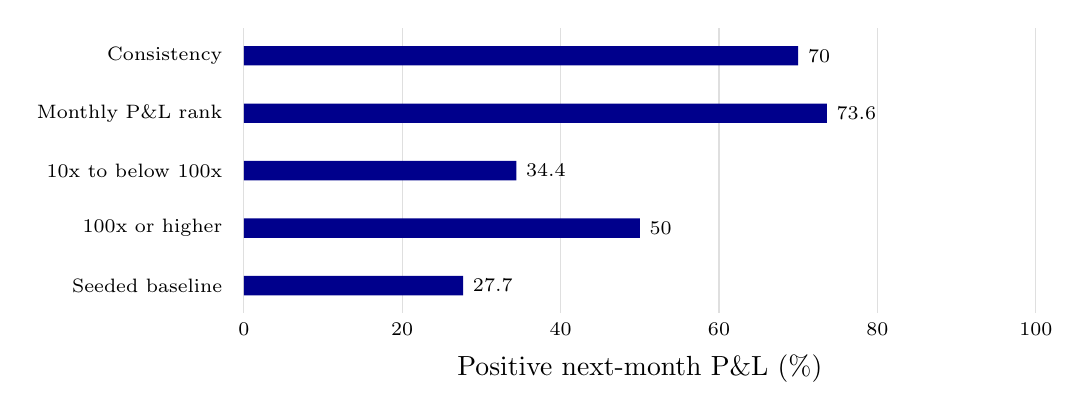
\begin{tikzpicture}
\begin{axis}[
  xbar, width=0.96\columnwidth, height=5.2cm,
  xmin=0, xmax=100, xlabel={Positive next-month P\&L (\%)},
  symbolic y coords={Consistency,Monthly P\&L rank,10x to below 100x,100x or higher,Seeded baseline},
  ytick=data, y dir=reverse, yticklabel style={font=\scriptsize},
  xtick={0,20,40,60,80,100}, x tick label style={font=\scriptsize},
  nodes near coords, nodes near coords style={font=\scriptsize},
  bar width=7pt, xmin=0, enlarge y limits=0.12,
  axis line style={draw=none}, tick style={draw=none},
  xmajorgrids=true, grid style={gray!25},
]
\addplot[fill=blue!55!black,draw=none] coordinates {
  (70.0,Consistency) (73.6,Monthly P\&L rank) (34.4,10x to below 100x) (50.0,100x or higher) (27.7,Seeded baseline)
};
\end{axis}
\end{tikzpicture}
\caption{Positive next-month trader P\&L frequency. The $100\times$ cohort contains only four rows.}
\label{fig:rates}
\end{figure}

The consistency screen is 42.3 percentage points above the seeded baseline, but 3.6 points below the largest-monthly-P\&L comparator. Their row-level Wilson intervals overlap. The intervals in Table~\ref{tab:cohorts} assume independent Bernoulli observations; repeated wallet-month rows violate that assumption, so they are descriptive uncertainty bands only. No significance test or causal claim is made. The $100\times$ estimate is highly uncertain because $n=4$.

Daily realized P\&L is not account ROI because full opening equity, bankroll, and cash-flow histories are unavailable. Large-multiple settled buys are exploratory cohorts and do not demonstrate persistent skill.

\begin{figure}[t]
\centering
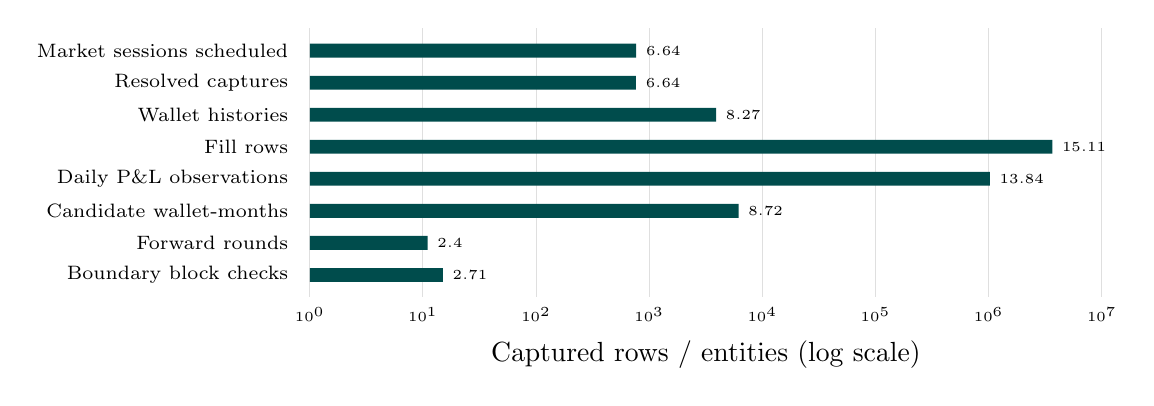
\begin{tikzpicture}
\begin{axis}[
  xbar, width=0.96\columnwidth, height=5.0cm,
  xmode=log, xmin=1, xmax=10000000,
  xlabel={Captured rows / entities (log scale)},
  symbolic y coords={Market sessions scheduled,Resolved captures,Wallet histories,Fill rows,Daily P\&L observations,Candidate wallet-months,Forward rounds,Boundary block checks},
  ytick=data, y dir=reverse, yticklabel style={font=\scriptsize},
  xtick={1,10,100,1000,10000,100000,1000000,10000000},
  xticklabel style={font=\tiny}, nodes near coords,
  nodes near coords style={font=\tiny}, bar width=5pt,
  axis line style={draw=none}, tick style={draw=none},
  xmajorgrids=true, grid style={gray!25},
]
\addplot[fill=teal!60!black,draw=none] coordinates {
  (768,Market sessions scheduled) (764,Resolved captures) (3906,Wallet histories)
  (3647433,Fill rows) (1025654,Daily P\&L observations) (6155,Candidate wallet-months)
  (11,Forward rounds) (15,Boundary block checks)
};
\end{axis}
\end{tikzpicture}
\caption{Polymarket capture scale by dataset object. The logarithmic axis is used because the object counts differ by several orders of magnitude.}
\label{fig:coverage}
\end{figure}

\section{Cross-Market Trader Data Study}
More records do not automatically imply better credit evidence. Venue-specific identity, currency, trade settlement, and permission models differ. Table~\ref{tab:venues} distinguishes public address-level history, owner-authorized account history, non-cash research records, and market-data infrastructure. Only Polymarket is currently in AQRA's measured benchmark; no extra venue sample is claimed.

\begin{table*}[t]
\caption{Prediction-market trader data access reviewed for AQRA}
\label{tab:venues}
\centering
\small
\begin{tabularx}{\textwidth}{lXXX}
\toprule
Venue & Trader-level data & Access/completeness constraint & AQRA treatment\\
\midrule
Polymarket & Public wallet P\&L, positions, activity, trade endpoints & Address can be proxy/deposit account; source coverage and wallet linkage need auditing & Current benchmark and borrower evidence source \cite{polymarket-pnl}\\
OPINION & Filled wallet trades, positions, fees, quote token and USD value & API key; paginated address history & Priority cash-market adapter after full pagination, fee and settlement validation \cite{opinion-trades,opinion-positions}\\
Predict.fun & Address-level fills, positions, activity; BNB trade, resolution and settlement events & Mainnet API key; smart-account ownership; independent archive begins 22 Oct 2026 & Priority short-window replication; preserve recent-only history and verify complete replay \cite{predict-api,predict-activity,predict-matches,bitquery-predict}\\
Limitless & Account positions, AMM/CLOB trades, and portfolio activity history & Authenticated owner account with HMAC signing; indexer state should reconcile to chain & Opt-in account adapter; not a public trader census \cite{limitless-api}\\
Kalshi & Public markets; member-specific orders, trades and portfolio & Signed member key; account-specific access and data-use limits & Member-consented data only, subject to permission and secure credential handling \cite{kalshi-keys,kalshi-developer,kalshi-data}\\
Gemini Predictions & Public markets and aggregate volume; private positions and order history & Authenticated API/OAuth; no public trader census & Opt-in account data after historical-settlement completeness review \cite{gemini-prediction,gemini-position}\\
Manifold & Public bets, user and portfolio history & M\$ virtual currency; free bulk data is non-commercial and last updated July 2024; commercial data licensing offered & Separate behavioral research cohort, never pooled into cash-credit policy without license and economic validation \cite{manifold-api,manifold-data}\\
Prediction.com & Matched events and market prices across covered venues & API key; supplies market, not wallet-trader histories & Event matching and price discovery only; not another trader cohort \cite{prediction-aggregator}\\
Bitquery & Decoded Polygon and BNB fills, resolutions and settlements & Provider API; Predict.fun real-time data only from 22 Oct 2026, with no archive & Independent chain reconciliation; deduplicate against venue APIs \cite{bitquery-pm,bitquery-predict}\\
\bottomrule
\end{tabularx}
\end{table*}

The next direct cash cohorts are OPINION and Predict.fun. OPINION provides wallet-level filled trades and positions behind an API key. Predict.fun exposes wallet-address activity and fills through an API and has BNB on-chain trade and settlement coverage, but only a recent indexed window; it supports a short-window replication, not the same 12-month walk-forward period. Limitless, Kalshi, and Gemini require account-owner authorization and cannot create a public trader census. Manifold supports a separate virtual-currency behavioral check subject to commercial licensing. Prediction.com can match markets and prices; Bitquery can independently decode supported chain events. Neither is a new trader population. No additional venue data have been collected into AQRA's benchmark because provider credentials and permissioned account exports are not configured in this checkout.

An adapter must preserve raw source units and supply a consented stable identity, point-in-time trade/fill timestamps, price/size/fees, settlement status, cash-flow history, open exposure and a reproducible cutoff. P\&L must separate realized cash outcomes from unrealized marks, rewards, rebates, deposits, transfers and volume. Each venue requires its own walk-forward sample, gap report, temporal split, and trader-clustered uncertainty before any pooled analysis.

\section{Credit Risk and Binding Gate}
For loan $i$, let $EAD_i$ be principal outstanding, $B_i$ the bond, and $h\in[0,1]$ an assumed bond recovery fraction, following the conventional exposure-at-default, probability-of-default, and loss-given-default decomposition \cite{basel-credit}. Principal loss after recovery is
\begin{equation}
\ell_i=\max(0,EAD_i-hB_i), \qquad EL=\sum_i PD_i\ell_i.
\end{equation}
The prototype's \(PD_i\), pairwise correlation, recovery haircut, capital charge, operating cost, and hypothetical reserve are scenario inputs. Trader P\&L does not calibrate any of them.

For a homogeneous group of $N$ loans with marginal default scenario $p$ and pairwise default-indicator correlation $\rho$, the engine uses a beta-binomial default count for $0<\rho<1$:
\begin{align}
\alpha &=p\frac{1-\rho}{\rho}, & \beta &=(1-p)\frac{1-\rho}{\rho},\\
\Pr(K=k)&={N\choose k}\frac{B(k+\alpha,N-k+\beta)}{B(\alpha,\beta)},\quad k=0,\ldots,N.
\end{align}
The $\rho=0$ and $\rho=1$ cases use binomial and common-shock limits. VaR is the discrete loss quantile. Expected Shortfall includes fractional probability mass at its tail boundary \cite{rockafellar-uryasev}. The application keeps pooled credit approval rejected until mature loan outcomes, calibrated PD, out-of-time validation, and committed capital exist.

A future validation must split by origination date; avoid wallet and regime leakage; label only matured loans; separate late, partial, default, and censored records; and report calibration, Brier score, log loss, observed-to-expected defaults, recovery and uncertainty. Trader P\&L is not a substitute for any loan label.

\section{Arkiv and Evidence Status}
Arkiv Rabdi is the lender-discovery layer for the \texttt{aqra.trader.credit.v2} schema. Swarm stores the exact borrower-consented report. The EVM contract stores debt, bond, lifecycle state, and report commitment. The lender discovers a pointer, retrieves report bytes, recomputes evidence, and verifies the pointer against contract state before funding.

On 6 November 2026, the current checkout queried the public Rabdi endpoint with the implemented schema and received zero current AQRA credit entities. The SDK warned that no access key is configured and the public endpoint is rate limited \cite{arkiv-rabdi,arkiv-entity}. This is evidence of a successful public read only; no borrower write receipt, public transaction hash, or second-wallet read proof is recorded. No Bee URL or funded postage batch is configured, so fresh report publication and report-backed funding are unavailable from this workspace until Swarm is configured \cite{swarm-upload}. A funded Rabdi wallet with tGLM is also needed to publish an entity.

The Chainlink CRE workflow source exists, but no successful public CRE/DON execution receipt is recorded \cite{chainlink-cre}. Local report-forwarder output must not be described as a public oracle execution.

\section{Limitations and Conclusion}
AQRA's benchmark is sampled, the wallet-month rows are dependent, and the winning screen does not beat the stronger prior-month P\&L comparator. The data include no starting account equity, full cash flow, or AQRA repayment labels. Consequently the present performance score is a reviewable eligibility screen, not proof of creditworthiness. The lender remains exposed to loss beyond the bond, and the prototype provides no position custody or production liquidity pool.

The next evidence milestones are (1) complete a consented, API-key-backed OPINION adapter and compare it as a separate cohort; (2) record the first real Rabdi entity write and independent query; (3) configure Swarm and complete a report-backed borrower-to-lender test; and (4) collect matured AQRA repayment outcomes before estimating PD. These steps strengthen the evidence chain without asserting that trading profit guarantees repayment.

\bibliographystyle{IEEEtran}
\bibliography{references}
\end{document}
